
\chapter{相关研究综述}
\label{chap:relatedwork}
流行度预测问题自被提出以来,受到了学术界和产业界的广泛关注。本章从流行度的统计特征分析、流行度预测方法以及流行度预测问题的可预测性三个方面入手,对流行度预测领域的相关工作进行了系统的总结和归纳,以便读者更好地了解和掌握该领域的相关知识,进而更好地理解本文的工作。

\section{流行度的统计特征分析}
在线内容的流行度分析工作最早源于网站缓存策略的研究。Cunha等人\citep{cunha1995characteristics}在研究站点中网页的访问情况时发现,网页被访问频率的分布服从Zipf定律\citep{zipf2016human},也就是说:流行度排名为$i$的网页被用户访问的概率正比于$1/i$,如图\ref{fig:pageDist}所示。这一现象表明,网页的访问频次分布是不均匀的。Almeida等人\citep{almeida1996characterizing}在研究万维网中所有网页的访问频次时,也发现了同样的分布规律。
\begin{figure}[!htbp]
  \centering
  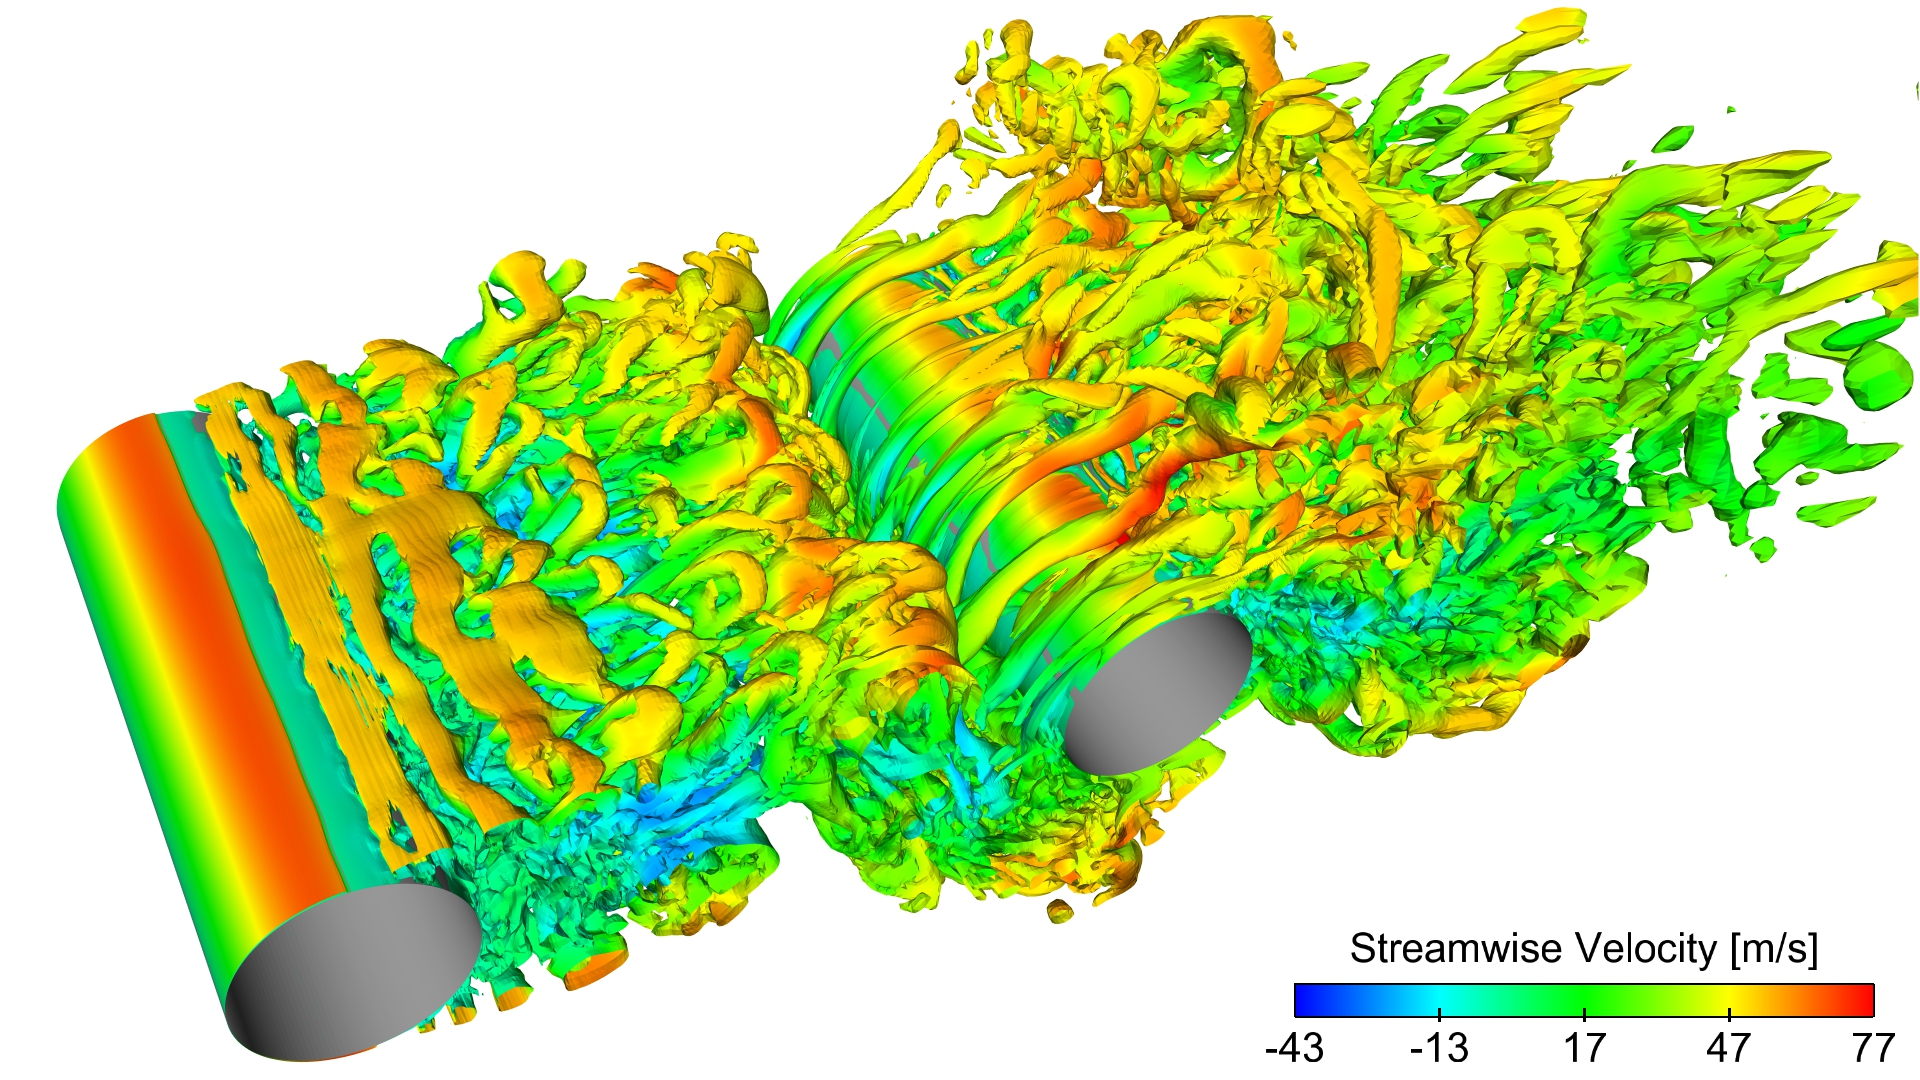
\includegraphics[width=0.45\textwidth]{ITC_Q_Criteria}
  \caption{Q判据等值面图}
  \label{fig:pageDist}
\end{figure}

随着信息技术的发展,视频分享类网站和社交网络平台不断涌现,也引起了研究人员的关注。Gill等人\citep{gill2007youtube}收集并分析了视频网站Youtube\footnote{\url{https://www.youtube.com}}上视频的访问数据,发现视频的访问频次信息依然服从Zipf定律。Cha等人\citep{cha2009analyzing}对Youtube网站上的视频数据进行了详细的分析,发现网站中不同类别下的视频的观看数分布都服从幂律分布。Kwak等人\citep{kwak2010twitter}研究了社交网络平台Twitter\footnote{\url{https://twitter.com}}上消息的转发情况,发现参与消息转发的人数服从幂律分布,如图\ref{fig:tweetDist}所示。
\begin{figure}[!htbp]
  \centering
  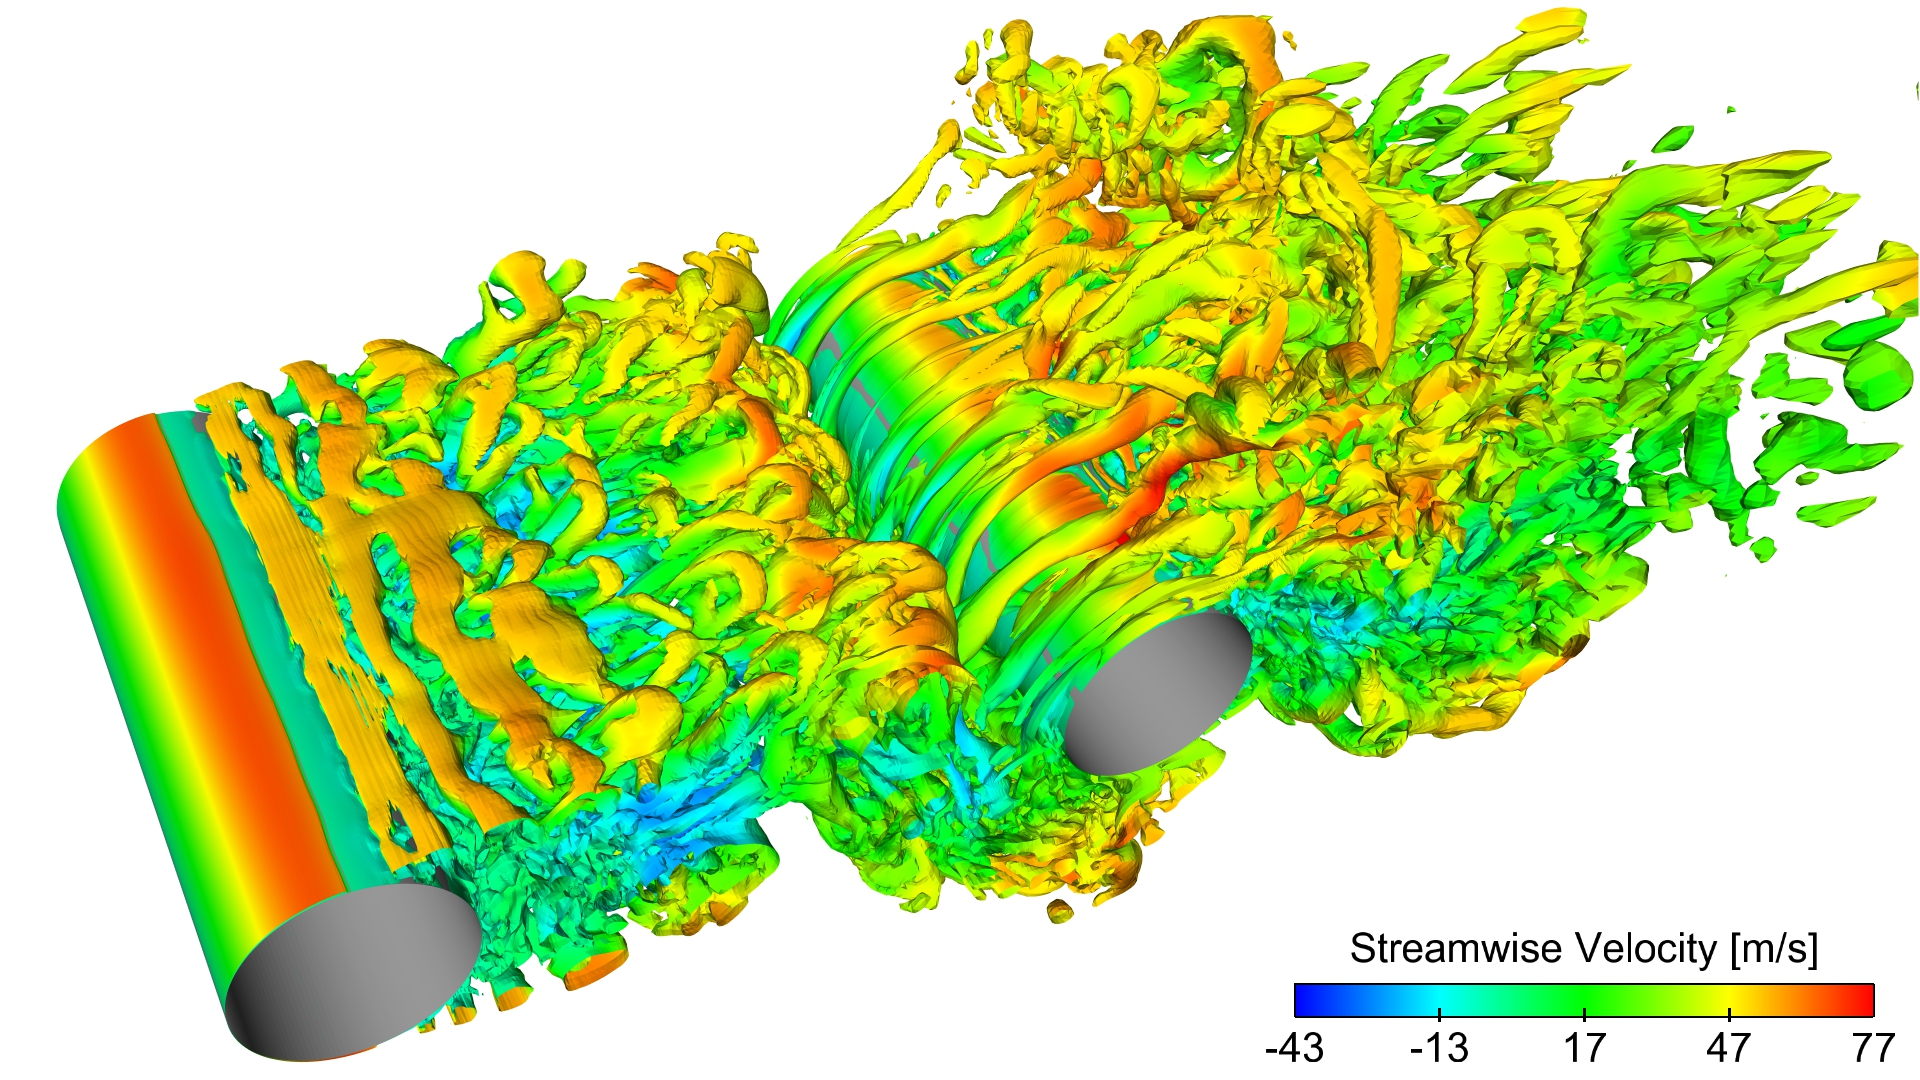
\includegraphics[width=0.45\textwidth]{ITC_Q_Criteria}
  \caption{Q判据等值面图}
  \label{fig:tweetDist}
\end{figure}

除了对宏观的流行度统计量的分析之外,还有一部分工作研究了流行度增长过程中的微观统计特征。Barabasi等人\citep{barabasi05}研究了人类的行为数据,发现人类的行为模式并不是服从传统方法中假设的泊松过程,而是存在爆发现象,并提出了一种基于事件优先级的排队模型来解释这一现象。爆发现象是指人类在参与某类事件时,大部分时间都处于沉寂状态,不会采取任何行为动作;中间夹杂了少数爆发区域,在爆发区域内会有大量的行为数据产生,如图\ref{fig:burst}所示。

爆发现象在在线内容的流行度增长过程中十分常见。Kaltenbrunner等人\citep{kaltenbrunner2007description}研究了新闻评论网站Slashdot\footnote{\url{https://slashdot.org}}上新闻的评论情况,并对评论数据的时间间隔分布进行了分析。统计结果表明,评论数据的时间间隔分布是两个log-normal分布的混合,并且存在明显的周期现象。Bao等人\citep{bao2013cumulative}研究了新浪微博中消息的转发时间间隔数据,发现转发时间间隔分布服从幂律分布,这也说明了社交网络中消息的流行度累积过程中存在爆发现象。
\begin{figure}[!htbp]
  \centering
  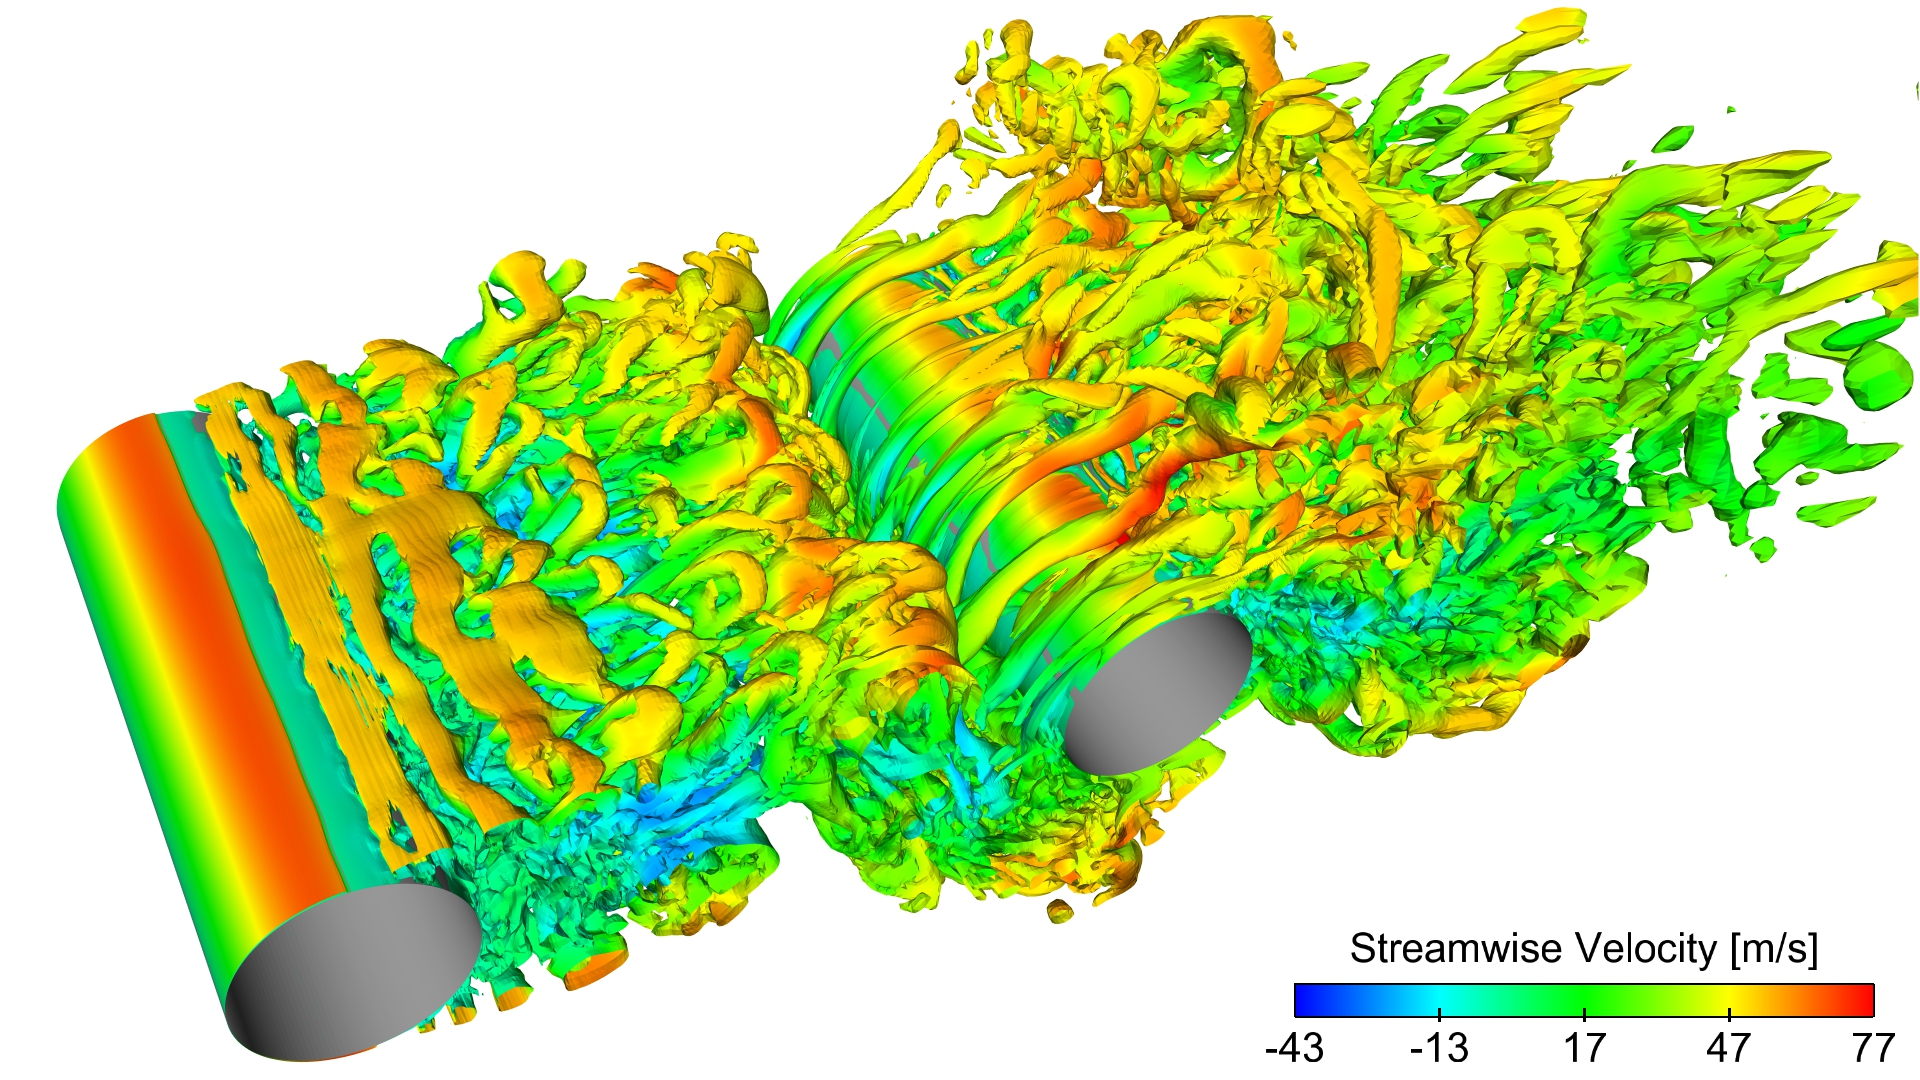
\includegraphics[width=0.45\textwidth]{ITC_Q_Criteria}
  \caption{Q判据等值面图}
  \label{fig:burst}
\end{figure}

除爆发现象外,研究人员还发现流行度的增长过程中存在着固定的模式。Yang等人\citep{yang2011patterns}研究了Twitter平台上消息的传播过程,提出了K-SC(K-Spectral Centroid)聚类方法,对消息的流行度变化过程进行聚类,将消息的流行度变化过程聚为六类,如图\ref{fig:pattern}所示。Crane等人\citep{crane2008robust}在研究Yotube网站中视频的观看数据时发现,视频的观看到达时间服从幂律分布,呈现出明显的``爆发-衰落"现象。此外,Costa等人\citep{ferraz2015rsc}还发现流行度的增长过程中呈现出明显的周期性特点。
\begin{figure}[!htbp]
  \centering
  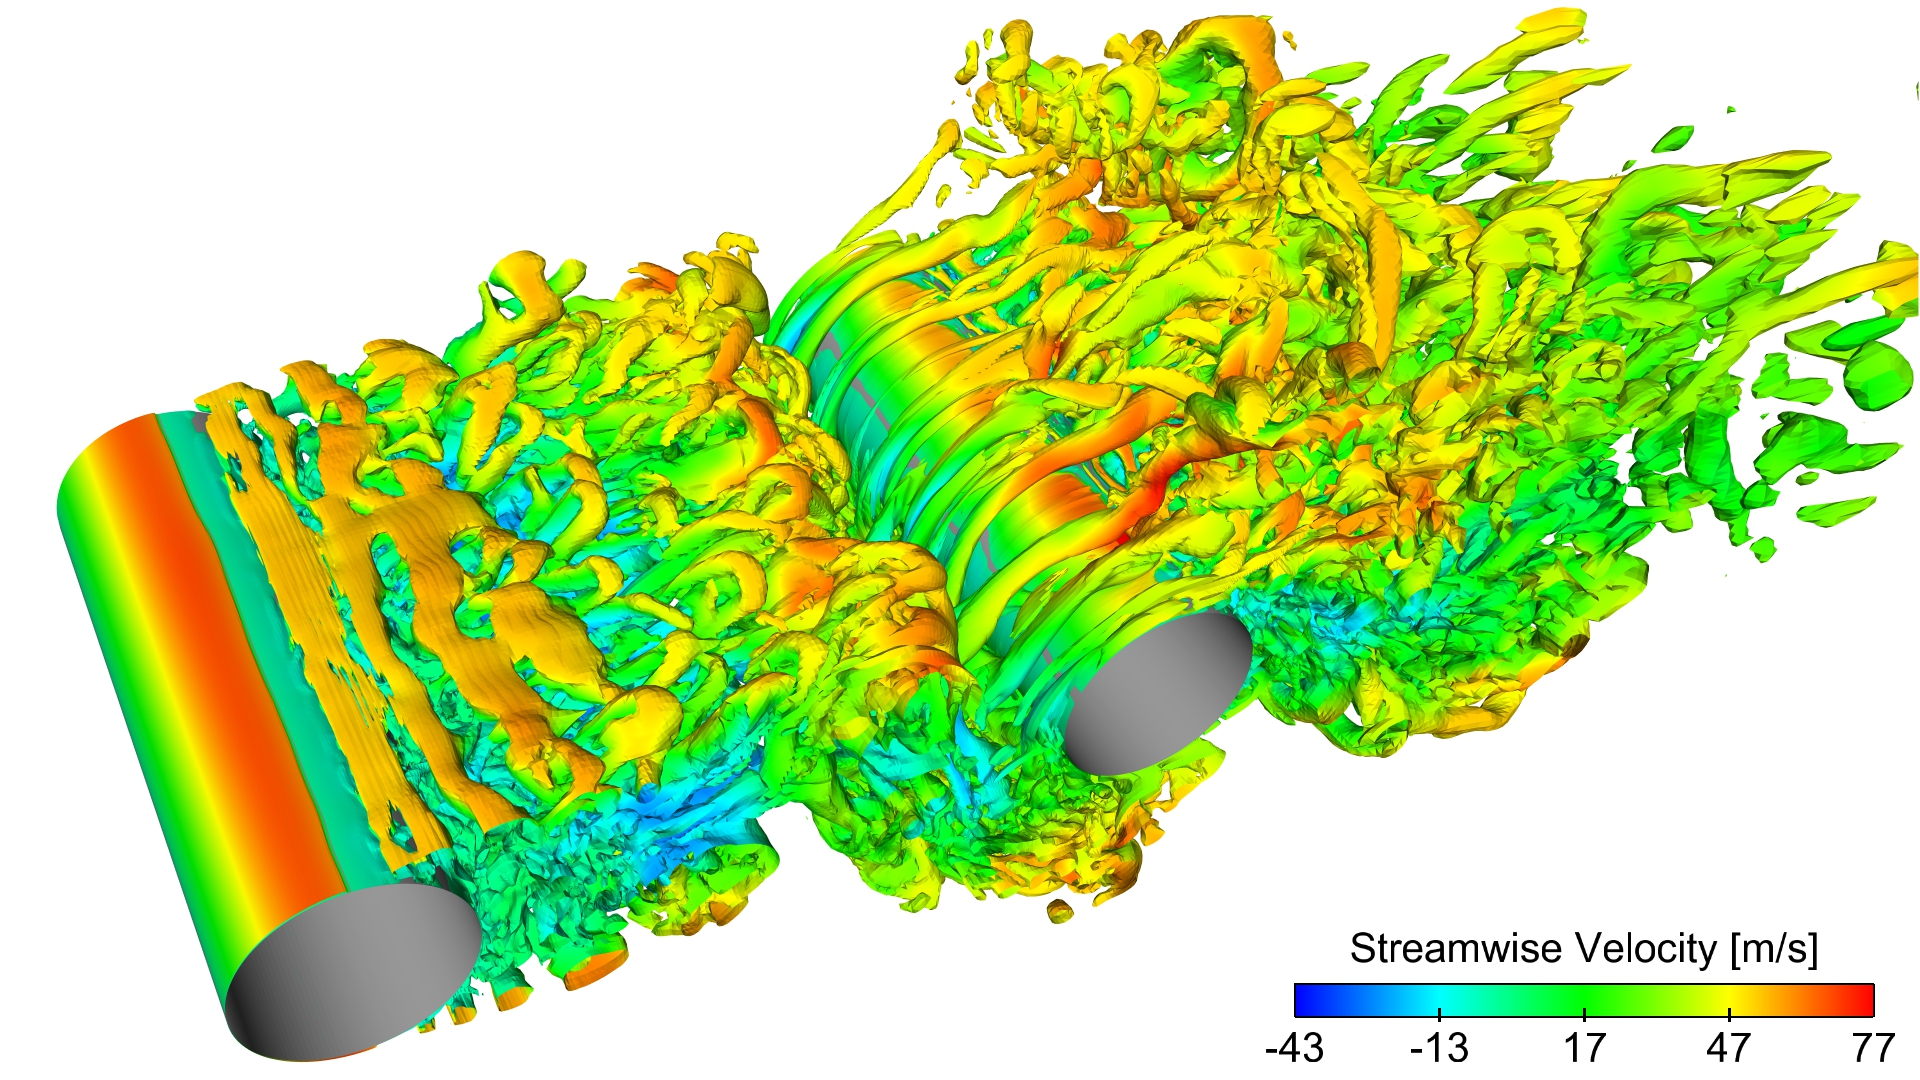
\includegraphics[width=0.45\textwidth]{ITC_Q_Criteria}
  \caption{Q判据等值面图}
  \label{fig:pattern}
\end{figure}

流行度分布的不均匀性,以及增长过程出现的爆发现象和时序特性,吸引了大量研究人员的关注,进而涌现出了多种流行度预测的模型和方法。
\section{流行度预测方法概述}
现有的流行度预测方法主要包含三类:基于特征的有监督学习方法、基于随机过程的流行度到达过程建模方法和基于表示学习的方法。本节会依次对这三类方法进行介绍和总结。
\subsection{基于特征的有监督学习方法}
基于特征的流行度预测方法主要通过借助已有的有监督学习模型,结合人工抽取的特征,来对流行度的增长过程进行预测。在这类方法中,流行度预测问题通常会被形式化为分类或者回归问题:给定一组历史消息的各种特征信息以及消息在观测窗口$[0,T_r]$和预测窗口$[0,T_s]$内的流行度数据作为训练样本,利用现有的分类或回归方法学习得到预测模型,进而对待预测的消息的流行度作出预测。这类方法的核心在于寻找对于流行度预测有着重要指示作用的特征。常见的用于流行度预测的特征包括消息内容特征、用户特征、时序特征和传播级联的结构特征。
\begin{figure}[!htbp]
  \centering
  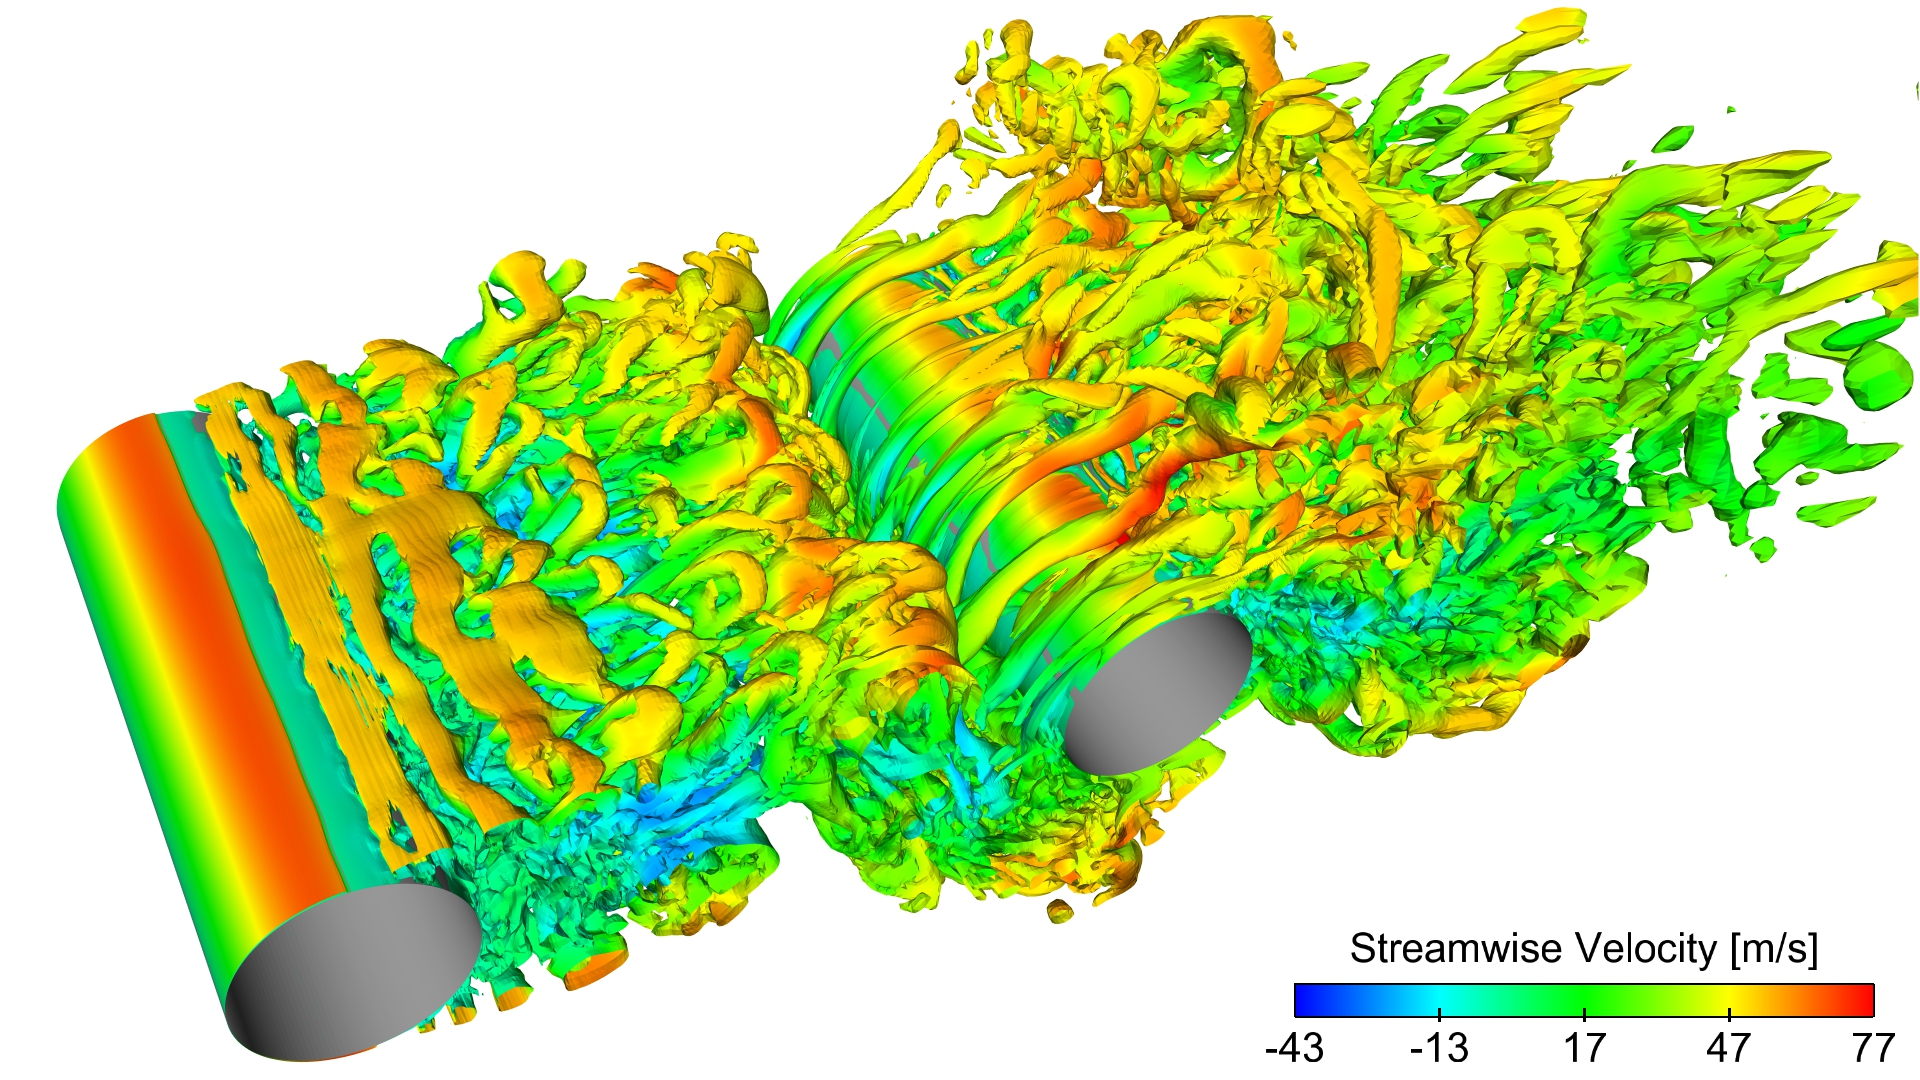
\includegraphics[width=0.45\textwidth]{ITC_Q_Criteria}
  \caption{Q判据等值面图}
  \label{fig:loglinear}
\end{figure}

时序特征方面,常用于流行度预测的时序特征包括观测窗口内的累积流行度特征和流行度时间序列特征。Cha等人\citep{cha2009analyzing}分析了Youtube网站上视频的流行度增长数据,发现视频上传7天后的访问量和视频上传后一天以及上传后两天的访问量之间存在着非常强的相关性,进而提出了预测视频近期流行度的任务,并指出视频上传后短期内的累计流行度是重要的指示特征。Szabo等人\citep{szabo2010predicting}研究了Digg\footnote{\url{http://digg.com}}网站上的新闻数据和Youtube网站上的视频数据,发现这些内容早期的流行度和后期的流行度在进行对数变换后,存在着非常强的线性相关性,如图\ref{fig:loglinear}所示。基于这一观测,作者提出了S-H(Szabo-Huberman)模型,将消息在观测窗口内的累积流行度作为特征,利用对数线性回归模型来预测消息在预测时刻的流行度。Gursun等人\citep{gursun2011describing}分析了Youtube网站中部分视频在上传后一年内完整的观看频次序列,发现可以根据将视频按照访问频次分为两类:长期流行的视频和短期流行的视频,并利用时间序列分析模型中的自回归移动平均模型(Autoregressive Moving Average,ARMA)\citep{marple1987digital},对长期流行的视频的流行度变化过程进行了预测。Pinto等人\citep{pinto2013using}研究了Youtube网站中视频的流行度时间序列数据。作者将视频在观测窗口等分为若干长度相等的区间,并抽取了各时间区间内视频的观看数的增长量作为特征。作者在研究视频的时间序列后发现S-H模型的假设存在着局限性:早期累计流行度相近的视频,后期的流行度变化过程可能会有很大的差距,如图\ref{fig:pinto}所示。作者提出将消息在观测窗口内的时间序列数据作为特征,利用多元线性回归模型来预测消息的流行度。
\begin{figure}[!htbp]
  \centering
  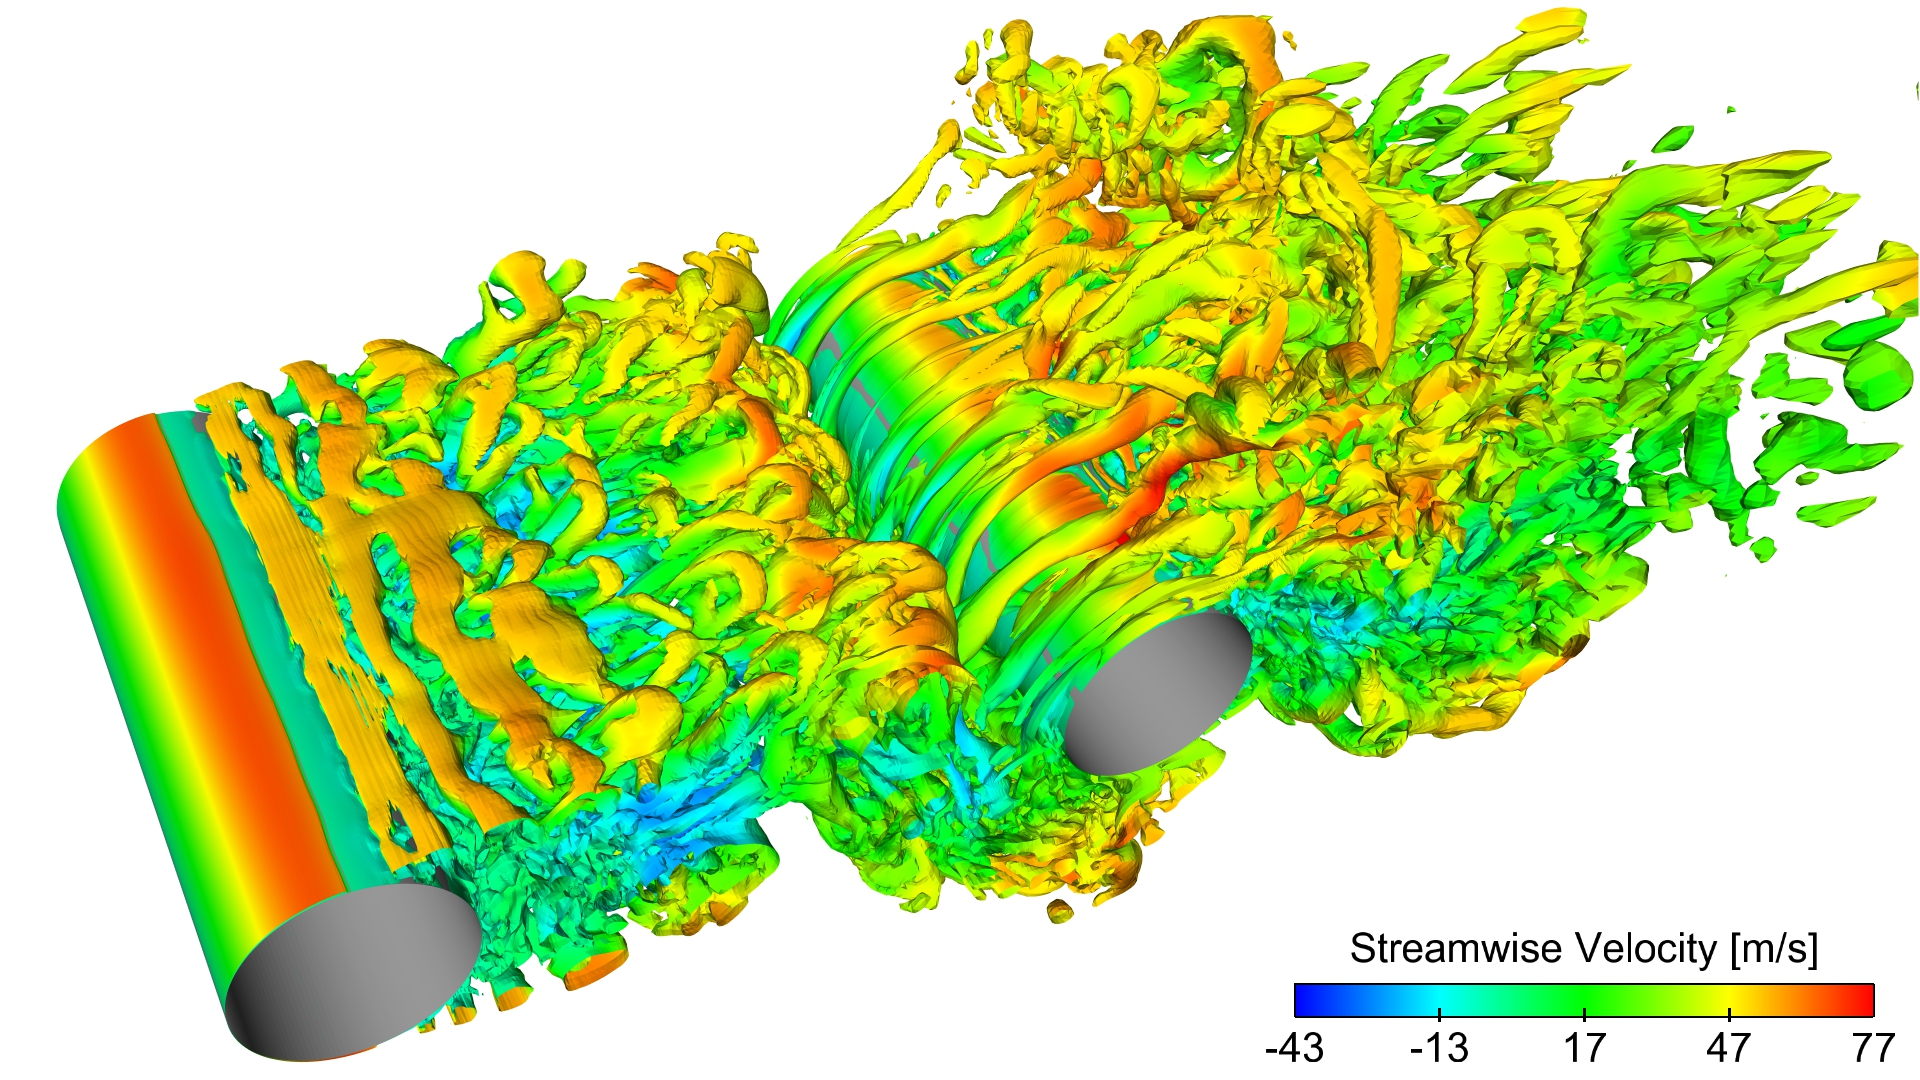
\includegraphics[width=0.45\textwidth]{ITC_Q_Criteria}
  \caption{Q判据等值面图}
  \label{fig:pinto}
\end{figure}

内容特征方面,Tsagkias等人\citep{tsagkias2009predicting}抽取了新闻的内容特征,来对新闻的评论数进行事前预测:在新闻发布之前,利用新闻的元信息,来预测新闻的评论数。作者将这一预测问题形式化为两阶段分类问题:新闻发布能否接收到评论,以及接收到的评论数会高还是低。在特征方面,作者抽取了新闻中重要性较高的前100个词的词频信息作为新闻的文本特征,新闻中包含的不同类型的命名实体的个数作为新闻的语义特征。此外,作者还抽取了新闻的其他元信息特征。实验结果表明,文本特征和语义特征对分类结果有较好的指示作用。Hong等人\citep{hong2011predicting}同样将Twitter平台中消息的流行度预测问题形式化为一个两阶段分类问题:消息是否会被转发以及消息最终的流行度等级。作者利用TF-IDF模型和LDA主题模型\citep{blei2003latent}来抽取消息的内容特征,同时结合网络拓扑结构特征以及时序特征来进行预测。Bandari等人\citep{bandari2012pulse}研究了新闻订阅站点Feedzilla\footnote{\url{http://news.feedzilla.com}}的数据在Twitter平台上的流行度情况。作者抽取了新闻的四类内容特征来进行预测,包括新闻所属的类别、新闻源站点的信息、新闻的倾向性特征和新闻中包含的命名实体。作者分别使用回归和分类模型对新闻的流行度进行了预测,得到了很好的预测效果。Bian等人\citep{bian2014predicting}研究了腾讯微博\footnote{\url{http://t.qq.com}}中消息的传播情况和用户的参与情况,从兴趣导向、社交影响和病毒式传播三个方面,建模了用户和消息之间的相互作用,进而对消息的流行度和用户的参与情况进行预测。建模过程中,作者提出了一种多任务迁移模型来建模消息的内容,提取出消息中的主题信息,用于后续的预测任务。

用户特征方面,最常见的用户特征是用户在社交网络中的拓扑结构信息,例如Twitter平台中用户的粉丝数和关注数信息\citep{gupta2012predicting,zhao2013short,kupavskii2013predicting,kong2014predicting}。用户的某些元信息也会被提取作为特征,包括用户账号的创建时长、用户历史发布的消息数\citep{suh2010want}、视频网站中的用户类别\citep{borghol2012untold}等。Yang等人\citep{yang2010modeling}在研究Twitter平台上消息的传播情况时,考虑了用户间的相互影响,提出了一种线性影响力模型。该模型可以在网络拓扑结构未知的情况下,来刻画用户间的影响力。Cui等人\citep{cui2013cascading}在研究Twitter平台上的消息爆发预测时,直接将用户身份作为特征。消息爆发预测问题旨在于给定消息在观测窗口内的流行度变化情况,预测消息最终的流行度能否达到爆发的阈值。作者在建模时借助于传感器的思想,将网络中所有的用户都当作传感器,只需要根据部分关键传感器的激活状态,即用户是否参与消息转发,就可以来判断消息最终能否爆发。因此,作者将爆发预测问题形式化为一个二分类问题,以所有的用户为特征,将用户在观测窗口内的激活状态转化成0-1向量作为输入,以消息最终的爆发情况作为输出,训练得到一个二分类器,进而对待预测的消息进行预测。

传播级联的结构特征方面,Bao等人\citep{bao2013popularity}分析了新浪微博中消息的传播级联情况,重点研究了传播级联形成的转发树的深度和链接密度情况,发现这两个特征与流行度的变化之间存在着非常强的相关性。作者将这两个因素加入到S-H模型中,发现预测精度得到了很大的提升。

除上述四类特征之外,研究人员还探寻了很多其他因素对流行度的影响。Brodersen等人\citep{brodersen2012youtube}研究了Youtube视频的观看数与地理因素之间的关系。Jenders等人\citep{jenders2013analyzing}研究了内容的情感倾向性对Twitter平台中消息转发数的影响。Weng等人\citep{weng2013virality}研究了流行度与网络的社区结构之间的关系,Junus等人\citep{junus2015community}也将社区结构因素建模到流行度预测模型中。此外,还有工作考虑了用户有限的关注度对流行度的影响\citep{hodas2012visibility,weng2012competition}。

问题形式化方面,不同于传统工作中将流行度预测形式化为一个回归或者分类问题,Cheng等人\citep{cheng2014can}将流行度预测问题形式化为阶段性的增长预测问题。作者指出,在以往的流行度分类预测问题中,由于流行度本身的分布是幂律的,导致各个类别样本数极度不均匀,从而影响最终的预测效果。因此,作者提出了``$kto2k$"问题:给定当前流行度为$k$的消息,预测它们最终的流行度能否增长到$2k$。基于样本集中流行度的分布,作者证明了提出的``$kto2k$"问题是一个均衡的二分类问题,并抽取了内容特征、用户特征、网络结构特征以及时序特征来进行预测。实验结果表明,随着$k$的增长,分类预测的准确率也在不断提高。

综上所述,基于特征的有监督学习方法在进行流行度预测时,关键在于抽取出能指示流行度变化的特征,但是特征工程是一项非常耗时耗力的工作,而且很大程度上受限于研究人员的先验认识。

\subsection{基于随机过程的流行度到达过程建模方法}
基于随机过程的流行度到达过程建模方法主要是在生存分析理论\citep{klein2005survival}的框架下进行的。这类方法中常见的流行度预测问题定义如下:给定一条消息$m$在观测窗口$[0,T]$内每一次转发的时间戳序列$C^m=\{t_i^m|0=t_0^m \le t_1^m \le...\le t_N^m \le T \}$作为输入,其中$N$表示消息$m$在观测窗口内总的转发次数,$t_i^m$表示消息$m$的第$i$次转发的转发时间与消息$m$的源发时间的间隔,最终的目标是预测后续流行度随时间的变化情况。这类方法通常将流行度的增长过程形式化为一个计数过程(Counting process)\citep{andersen1985counting}:用随机过程$\{N(t),t \ge 0\}$来刻画消息累积流行度随时间$t$变化的序列,其中$N(t)$取值是非负整数,且满足单调性:$N(s) \le N(t)\text{,} \forall s \le t$。在生存分析理论框架下,建模序列$N(t)$的关键在于对强度函数(Intensity function)的刻画。强度函数$x(t)$刻画了在给定历史信息$H_t=\{t_i|t_i < t \}$时,时间区间$[t,t+dt)$内有新事件发生的概率,即:
\begin{equation}
\label{eq:intensity}
P\{[t,t+dt)\text{内事件发生} | H_t\}=x(t)dt\text{。}
\end{equation}
用$dN(t)$来表示在时间区间$[t,t+dt)$内发生的事件数,它的期望可以用$\mathbb{E}_{dN(t) \sim \{0,1\}}[dN(t)|H_t]=x(t)dt$表示,从而可以得到计数序列$N(t)$与强度函数$x(t)$之间的关系如下:
\begin{equation}
\label{eq:differential}
\frac{\mathbb{E}[dN(t)]}{dt}=x(t)\text{。}
\end{equation}
在确定强度函数的形式和参数后,可以通过求解公式(\ref{eq:differential})中的微分方程,来确定计数序列$N(t)$的具体形式,进而对任意时刻$t$的计数值进行预测。

强度函数的形式通常由研究人员通过先验知识来确定,而具体的参数可以在生存分析理论框架下求取。生存分析理论常用于建模某一类事件发生的概率随时间的变化关系,例如患病病人的存活概率随时间的变化关系。在生存分析理论中,用随机变量$T$来表示事件发生的时刻,则概率$S(t)=P(T>t)$表示了事件到$t$时刻仍未发生的概率,因此被称为生存概率,而$F(t)=P(T \le t)=1-S(t)$则被称为累积死亡概率。累积死亡概率$F(t)$对应的密度函数$f(t)$可以通过如下求导的方式获得:
\begin{equation}
\label{eq:density}
f(t)=\frac{dF(t)}{dt}=\frac{P(t \le T < t+dt)}{dt}\text{。}
\end{equation}
在生存分析理论中,强度函数$x(t)$与密度函数$f(t)$的关系可以用如下公式表示:
\begin{eqnarray}
\label{eq:intensityTransform}
\begin{split}
x(t) & =\frac{P\{[t,t+dt)\text{内事件发生}|H_t\}}{dt}=\frac{P\{t \le T < t+dt|T \ge t\}}{dt} \\
& =\cfrac{\cfrac{P\{t \le T < t+dt\}}{P\{T \ge t\}}}{dt}=\cfrac{\cfrac{P\{t \le T < t+dt\}}{dt}}{P\{T \ge t\}}=\frac{f(t)}{S(t)}\text{。} 
\end{split}
\end{eqnarray}
将密度函数$f(t)$的定义$f(t)=F'(t)=(1-S(t))=-S'(t)$代入公式(\ref{eq:intensityTransform}),可以得到:
\begin{equation}
\label{eq:intensityDifferential}
x(t)=\frac{f(t)}{S(t)}=-\frac{S'(t)}{S(t)}=-\frac{d[lnS(t)]}{dt}\text{。}
\end{equation}
两边取积分,得到:
\begin{equation}
\label{eq:intensitySurvival}
S(t)=exp\{-\int_{0}^{t}x(t)dt\}\text{。}
\end{equation}
密度函数$f(t)$也可以通过如下公式由强度函数$x(t)$来表示:
\begin{equation}
\label{eq:intensityDensity}
f(t)=x(t)\ast S(t)=x(t) \ast exp\{-\int_{0}^{t}x(t)dt\}\text{。}
\end{equation}
由此可见,在生存分析理论框架下,事件发生的概率密度和生存概率都可以用强度函数表示出来。在给定观测数据后,可以通过极大似然估计的方式,求取强度函数中的参数,得到强度函数的具体形式。具体到流行度预测问题中,对于前述给定的时间戳序列$C^m$,可以定义它的似然函数如下:
\begin{equation}
\label{eq:likelihood}
\mathcal{L}\{C^m\}=P_0(T|t_N^m)\prod_{i=1}^{N}p_1(t_i^m|t_{i-1}^m)\text{,}
\end{equation}
其中$P_0(T|t_N^m)$刻画了从$[t_N^m, T]$时间区间内没有新的流行度到达的概率,$p_1(t_i|t_{i-1})$刻画了给定上一次转发时刻为$t_{i-1}^m$的情况下,下一次转发发生在$t_i^m$的概率。在生存分析理论框架下,这两个概率分别对应$[t_N^m, T]$区间内的存活概率和$t_i^m$时刻的概率密度。给定强度函数$x(t)$,这两个概率可以如下表示:
\begin{eqnarray}
\label{eq:eventProb}
\begin{split}
P_0(T|t_N^m) & =exp\{-\int_{t_N^m}^T x(t)dt\}\text{,}\\
p_1(t_i^m|t_{i-1}^m) & =x(t)\ast exp\{-\int_{t_{i-1}^m}^{t_i^m} x(t)dt\}\text{。}
\end{split}
\end{eqnarray}
因此,在给定序列$C^m$的情况下,结合公式(\ref{eq:likelihood})和公式(\ref{eq:eventProb}),就可以求出强度函数$x(t)$的具体形式,进而根据公式(\ref{eq:differential})对流行度后续增长情况做出预测。

鉴于计数过程和流行度增长过程的天然相似性,很多流行度预测的工作都是从随机过程的角度开展的。Wang等人\citep{wang2013quantifying}研究了论文的引用数增长情况。作者提出并论证了影响论文引用数增长的三个关键因素:论文本身的质量、论文自身吸引力的时效性以及论文累积引用数,并将这三个因素建模到论文引用数的增长过程中。作者提出的模型可以根据论文发表后10年内的引用信息,来预测后续20年论文引用数的增长情况。在该工作的基础上,Shen等人\citep{shen2014modeling}采用了自增强泊松过程(Reinforced Poisson process, RPP)\citep{pemantle2007survey}来建模论文的引用数增长情况。在建模引用序列的强度函数时,作者考虑了上述三个影响因素,给出如下的强度函数:
\begin{equation}
\label{eq:intensityRPP}
x(t)=\lambda f(t;\theta)i(t)\text{,}
\end{equation}
其中$\lambda$是对论文本身质量的度量;$f(t;\theta)$是一个时序释放函数,用于刻画论文的吸引力随时间的变化情况,$\theta$是时序释放函数的参数;$i(t)$是自增强函数,用于刻画论文引用中的``富者愈富"现象。在论文引用数据集上,作者选取了Log-normal函数作为时序释放函数,并将自增强函数$i(t)$定义为到$t$时刻为止的论文引用数。数据集上的实验结果表明,作者提出的自增强泊松过程模型(RPP模型)可以很好地刻画论文引用的到达过程。此外,作者还对模型中的参数引入了先验,进一步提升了模型的预测效果。Gao等人\citep{gao2015modeling}将RPP模型应用到微博平台上消息的转发数预测中。作者详细分析了微博平台中消息转发数据的特点,并对RPP模型中的时序释放函数和自增强函数的形式进行了相应的修正。此外,作者还分析了微博平台中时间的异质性,引入``微博时间"的概念来对微博平台中的物理时间进行映射,从而消除时间异质性对预测效果的影响。修正后的RPP模型在消息转发数预测任务上取得了非常好的效果。

Bao等人在\citep{bao2015modeling}中指出,RPP模型在建模过程中,是将消息传播当做一个单源传播的过程,没有考虑转发操作带来的激励作用,这样的建模方式不适用于微博平台上的转发数据,因为微博平台中用户间的转发行为会影响消息最终的转发数。因此,作者提出利用自激励Hawkes过程(Self-exciting Hawkes process, SEHP)来建模每次转发带来的激励作用。基于自激励Hawkes过程,作者提出了如下强度函数:
\begin{equation}
\label{eq:hawkesIntensity}
x(t)=v e^{-\beta t}+\alpha \sum_{j=1}^{j_{max}(t)} e^{-\beta(t-t_j)}\text{,}
\end{equation}
其中,$j_{max}(t)$刻画了到$t$时刻为止的转发次数,$v$是对消息本身吸引力的度量,$\alpha$刻画了每次转发带来的激励强度,函数$e^{-\beta t}$刻画了激励强度随时间的衰减效应。相比于RPP模型,SEHP模型能更好地捕获每次转发带来的影响,如图\ref{fig:sehp}所示。
\begin{figure}[!htbp]
  \centering
  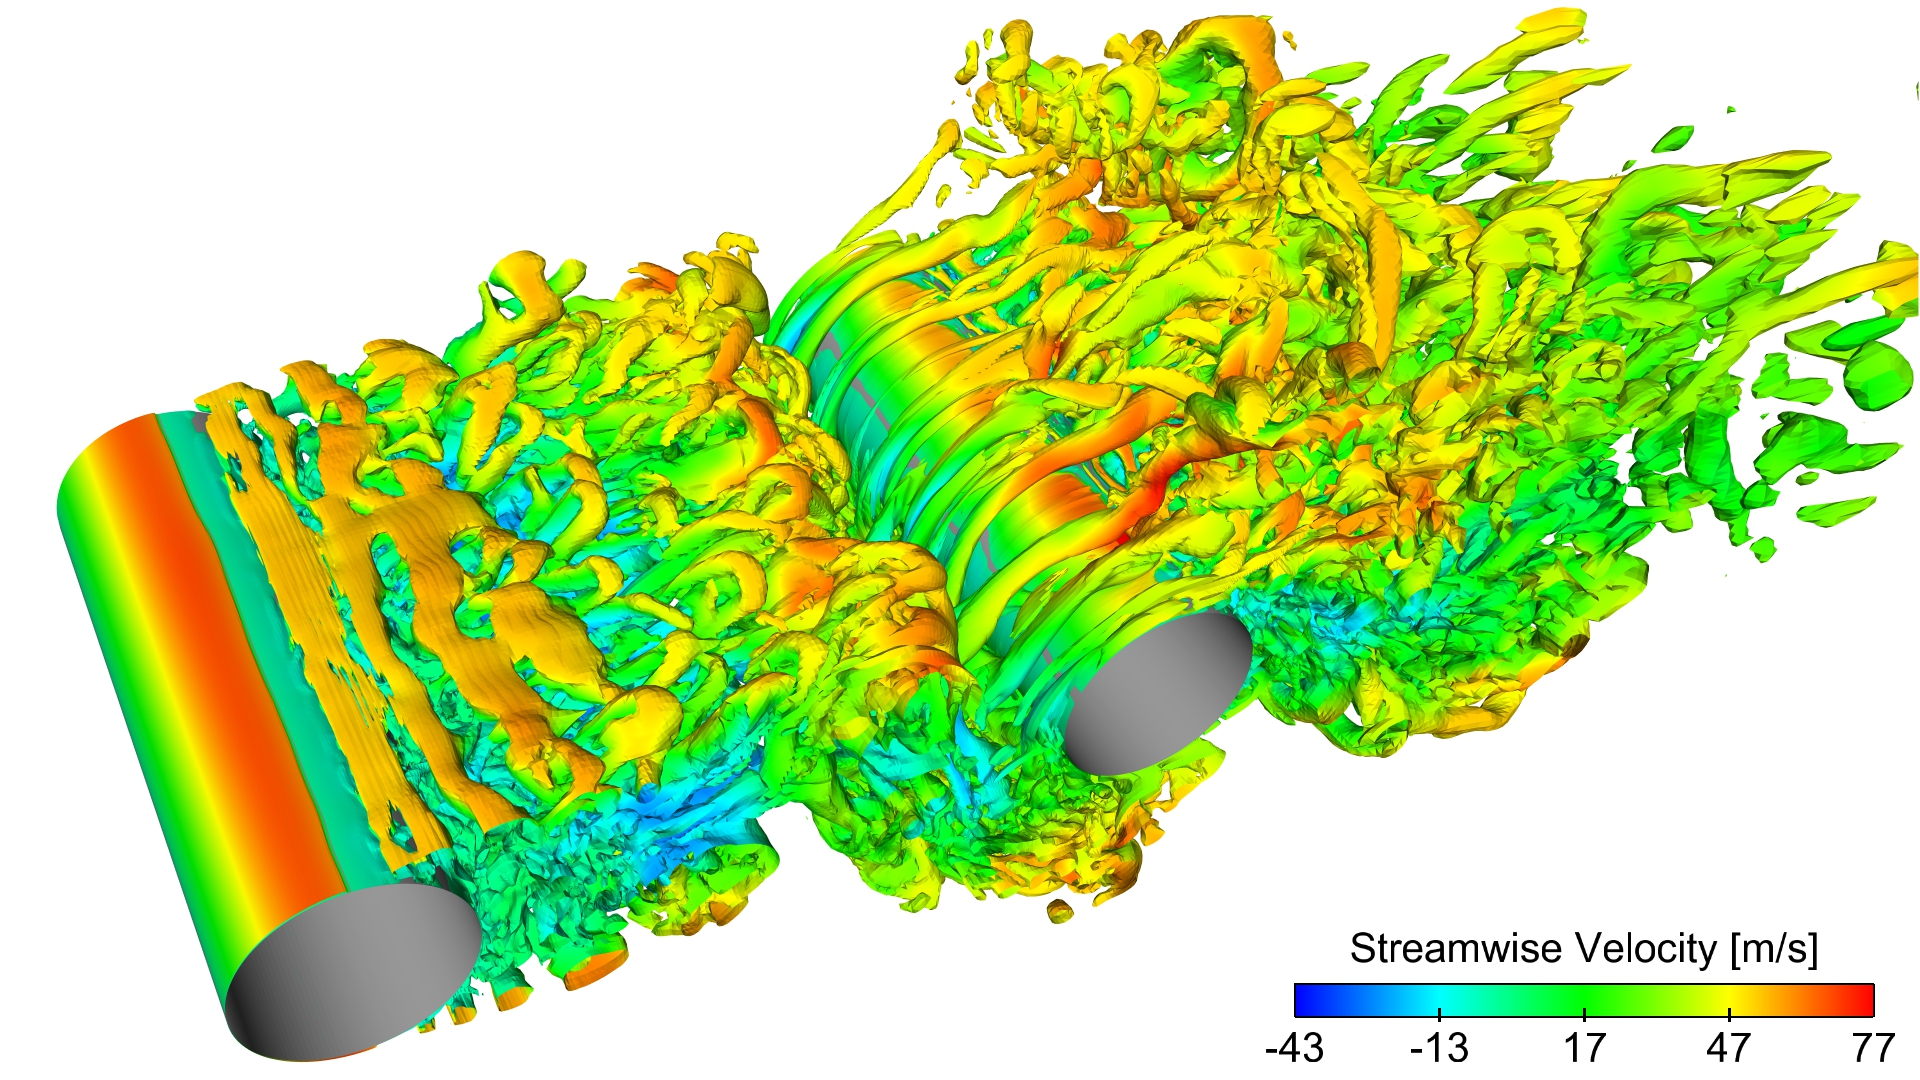
\includegraphics[width=0.45\textwidth]{ITC_Q_Criteria}
  \caption{Q判据等值面图}
  \label{fig:sehp}
\end{figure}
在该工作的基础上,作者还提出了ISEHP模型\citep{bao2016modeling},进一步考虑了不同转发用户带来的激励强度的差异以及微博平台上的时间异质性。

Zhao等人\citep{zhao2015seismic}研究了社交网络中消息爆发预测的问题。作者将爆发预测问题形式化为消息最终流行度的预测问题。作者同样采用了自激励Hawkes过程来建模消息流行度的转发过程。在建模用户激励强度时,作者引入了用户粉丝数,同时还将消息本身的感染力也建模成一个随机过程。最终作者给出流行度增长过程的强度函数如下:
\begin{equation}
\label{eq:seismic}
x(t)=p(t) \sum_{t_i<t}n_i \phi(t-t_i)\text{,}
\end{equation}
其中$p(t)$是用于刻画消息自身感染强度变化的随机过程,$n_i$是第$i$转发的用户的粉丝数,$\phi(t-t_i)$用于刻画感染强度随时间的变化关系。作者在论文中还指出,感染强度$p(t)$的大小反映了消息当前所处的增长状态:令$n^{\ast}$表示所有用户的粉丝数的平均值。当$p(t)>1/n^{\ast}$时,消息处于``超临界"状态,此时消息的流行度处于指数增长阶段,无法对消息的最终流行度做出预测;当$p(t)<1/n^{\ast}$时,消息处于``次临界"状态,此时消息的流行度增长状态逐渐减缓,可以预测消息的最终流行度。

在自增强泊松过程和自激励Hawkes过程在外,也有一部分工作采用了其他的随机过程来刻画流行度的增长情况。Lerman等人\citep{lerman2010using}研究了Digg网站上故事的得票数的变化情况。分析发现,故事在网站中的曝光度、故事本身的内容吸引力以及用户间的社会关系对故事最终的得票数有很大的影响。作者将这三个因素建模到故事得票数增长模型中,得到了很好的预测效果。Costa等人\citep{ferraz2015rsc}分别使用了使用泊松过程(Poisson process)\citep{kingman1993poisson}和自相关过程(Self-correlated process)来建模了消息的转发时间间隔的产生过程。Yang等人\citep{yang2013mixture}采用了多元Hawkes过程来建模多条消息的转发情况。Rizoiu等人\citep{rizoiu2017expecting}提出了Hawkes强度过程(Hawkes intensity process,HIP)来建模流行度时间序列的产生过程。Yu等人\citep{yu2015micro}研究了微博平台中消息的微观转发过程,并直接使用了生存分析理论来建模平台中用户发布的消息被自己的粉丝转发的概率。

纵观上述方法,基于随机过程的方法能够较好地刻画流行度的到达过程,但是由于是非监督学习的方法,它们的预测能力有限;同时流行度增长的强度函数的设计,很大程度上也依赖于研究人员的先验知识;另外,这类方法在建模过程中只利用了待预测消息自身的信息,没有显示地利用海量的历史消息来辅助提升预测性能。
\subsection{基于表示学习的方法}
表示学习目前已经发展成为一个重要的领域,在很多实际问题中都有着重要的应用。在流行度预测领域,
\subsection{其他方法}
\section{流行度预测问题的可预测性分析}

